\documentclass[8pt]{beamer}
\usetheme{metropolis}           % Use metropolis theme
\title{Unit 03 Preview}
\date{\today}
\author{Neo Wang}
\institute{Westlake High School}
\begin{document}
  \maketitle
  \begin{frame}{Table of Contents}
	\tableofcontents
  \end{frame}
  \begin{frame}
	\section{Aggregate Demand}
	The Wealth Effect
	\begin{itemize}
		\item \tiny Higher price levels reduce the purchasing power of money, which
		decreases the quantity of expenditures.
		\item \tiny Lower price levels increase purchasing power and increase
		expenditures
	\end{itemize}
	Interest Rate Effect
	\begin{itemize}
		\item \tiny When the price level increases, lenders charge higher interest to
		get a REAL return on their loans
	\end{itemize}
	Foreign Trade Effect
	\begin{itemize}
		\item \tiny When price levels rise, foreign buyers purchase fewer U.S. 
		goods and Americans buy more foreign goods. $X_n$ decreases.
	\end{itemize}
	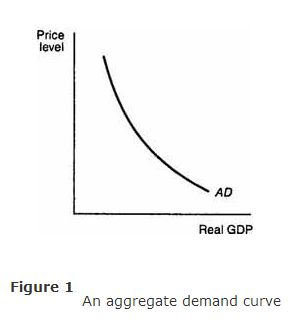
\includegraphics[width=2.5cm]{2021-10-12-11-50-24.png}
	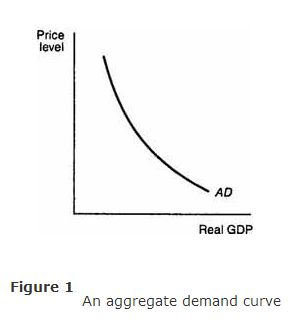
\includegraphics[width=2.5cm]{2021-10-12-11-59-30.png}
  \end{frame}
  \begin{frame}
	\section{Multipliers}
	\begin{itemize}
		\item Marginal Propensity to Save (MPS); How much people save instead of
		consume when there is a change in income. Expressed as $$MPS=\frac{\Delta \text{savings}}{\Delta \text {Disposable Income}}$$
		\item Marginal Propensity to Consume (MPC); How much people consume
		rather than saving when disposable income changes. Expressesed as a fraction:
		$$MPC = \frac{\Delta \text{consumption}}{\Delta \text{Disposable Income}}$$
		\item Spending Multiplier
		$$\frac{1}{MPS} = \frac{1}{1 - MPS}$$
		\item Simple Tax Multiplier
		$$\frac{MPS}{MPC}$$
		\center 
\includegraphics[width=2cm]{2021-10-12-12-10-06.png}
	\end{itemize}
  \end{frame}
  \begin{frame}
	\section{Short-Run Aggregate Supply (SRAS)}
	Things that can affect SRAS
	\begin{itemize}
		\item Change in the prices of resources
		\item Changes in taxes, subsidies, or regulations
		\item Change in productivity
		\item Expectations
	\end{itemize}
	$$Y = Y^* + \alpha(P-P_e)$$
	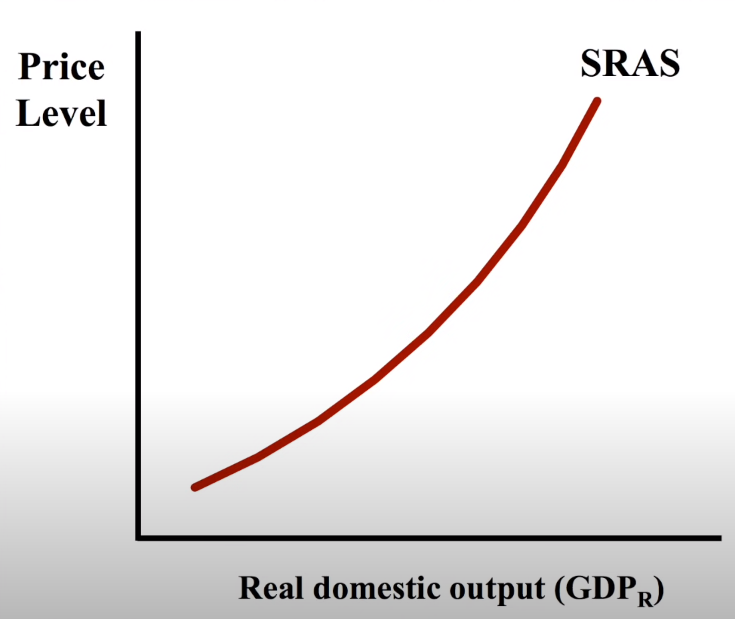
\includegraphics[width=2.5cm]{2021-10-12-12-11-36.png} 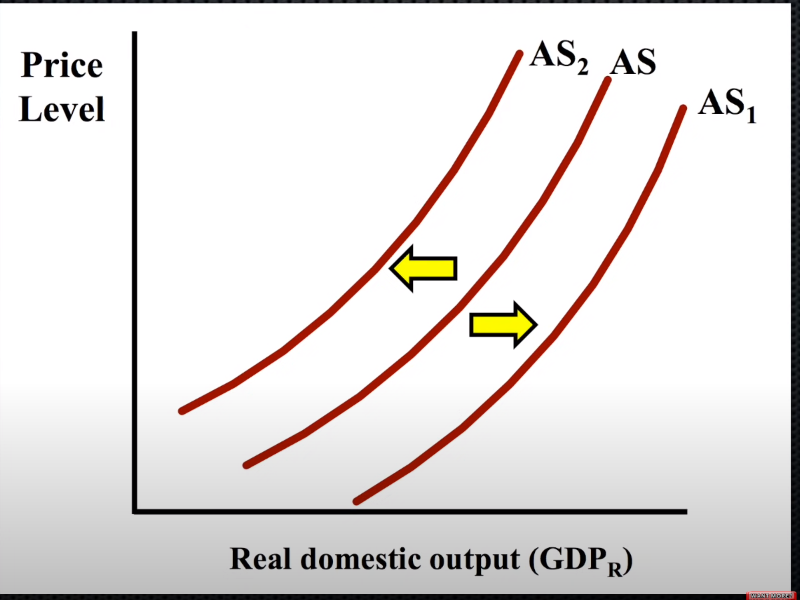
\includegraphics[width=2.5cm]{2021-10-12-12-12-26.png}
  \end{frame}
  \begin{frame}
	\section{Long-Run Aggregate Supply (LRAS)}
	\begin{itemize}
		\item The curve shows what we can produce at the natural rate of unemployment.
		\item A recessionary gap doesn't necessarily mean there's a recession.
		\item The curve shows relationship between price level and real GDP if
		everything was fully flexible. LRAS is vertical. 
	\end{itemize}
	$$Y = Y^*$$
	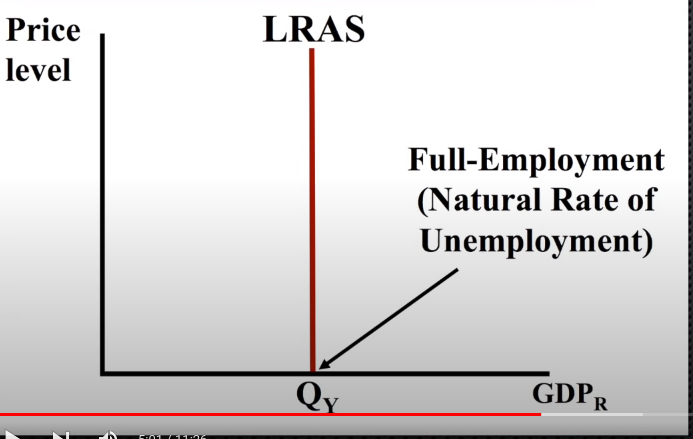
\includegraphics[width=2.5cm]{2021-10-12-12-18-10.png}
	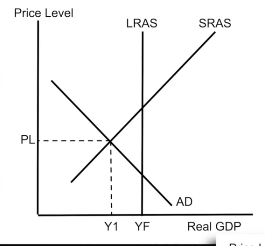
\includegraphics[width=2.5cm]{2021-10-12-12-58-09.png}
  \end{frame}
  \begin{frame}
	\section{Equilibrium in the Aggregate Demand-Aggregate Supply (AD-DS) Model}
	Overview
	\begin{itemize}
		\item Puts aggregate deamnd and aggregate-supply together.
		\item Recessionary gap doesn't necessarily mean there's a recession
	\end{itemize}
	Aggregate demand equation
	$$AD = C + I + G + (X - M)$$
	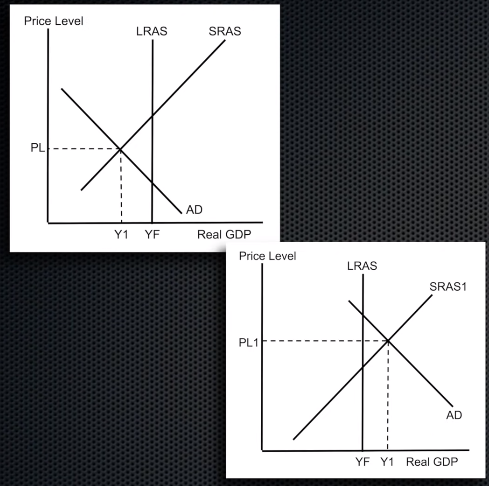
\includegraphics[width=2.5cm]{2021-10-12-12-45-18.png}
	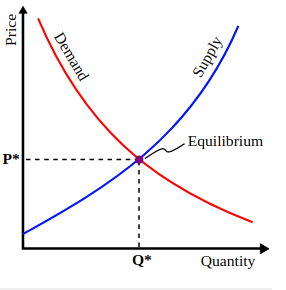
\includegraphics[height=2.5cm]{2021-10-12-13-03-25.png}
  \end{frame}
  \begin{frame}
	\section{Change in the AD-AS Model in the Short Run}
	\begin{itemize}
		\item This unit revolves around shifting curves, specifically SRAS, AD1
		\item Positive supply shock: the short supply increase.
		\item Cost push inflation, supply shifts left, and demand-pull shifts right.
	\end{itemize}
	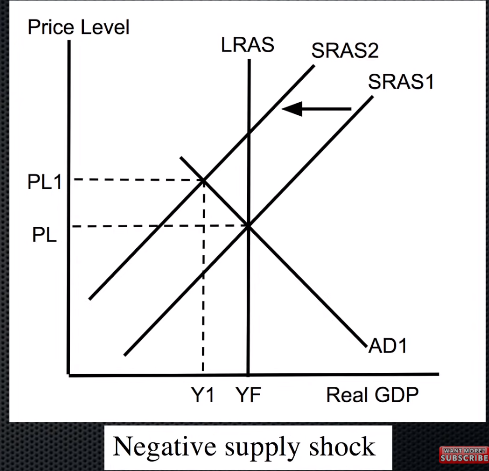
\includegraphics[height=2.5cm]{2021-10-12-12-47-38.png}
  \end{frame}
  \begin{frame}
	\section{Long-Run Self Adjustment}
	\begin{itemize}
		\item Idea that the economy self-adjusts; it's not demand that changes, it's shortened supply.
		\item If flexible, short ag will shift to the right, putting back at full employment.
	\end{itemize}
	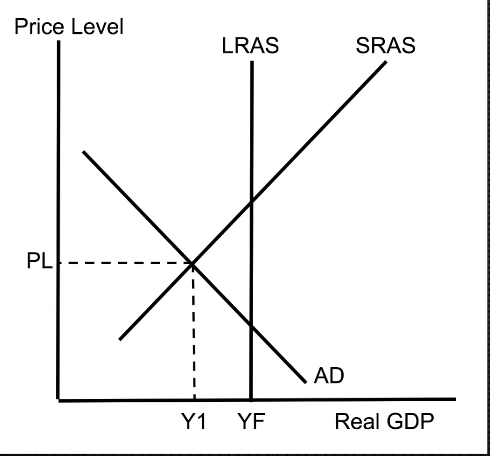
\includegraphics[height=2.5cm]{2021-10-12-12-49-20.png}
  \end{frame}
  \begin{frame}
	\section{Fiscal Policy}
	\begin{itemize}
		\item Government gets involved.
		\item Expansionary fiscal policy; laws that reduce unemployment and
		increase GDP; increaes spending, decrease taxes, combinations of the two.
		\item Contractionary fiscal policy; laws that reduce inflation, decrease GDP;
		decrease government spending, increase taxes, combinations.
	\end{itemize}
	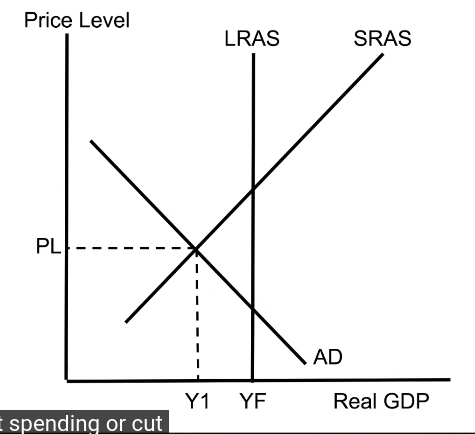
\includegraphics[height=2.5cm]{2021-10-12-12-51-33.png}
	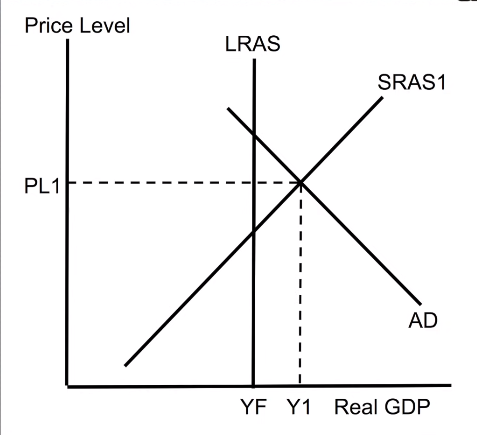
\includegraphics[height=2.5cm]{2021-10-12-12-51-48.png}
  \end{frame}
  \begin{frame}
	\section{Automatic Stabilizers}
	\begin{itemize}
		\item Discretionary fiscal policy; congress creates new bills that changes
		AD through spending
		\item Non-Discretionary fiscal policy; aka. automatic stabilizers.
		Permanent spending or taxation laws to work counter cyclically to
		stabilize the economy.
		\item When GDP goes down, government spending automatically increase, and taxes fall
	\end{itemize}
	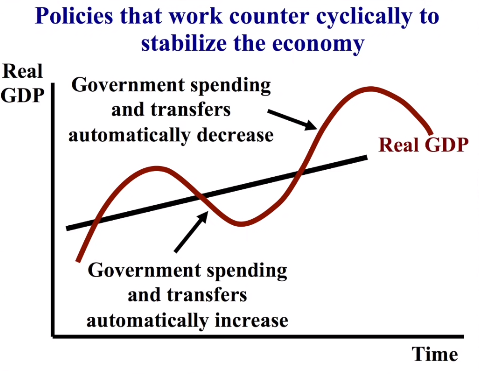
\includegraphics[height=2.5cm]{2021-10-12-12-56-27.png}
  \end{frame}
\end{document}